\section{MODELLING OF THE ECRH BEAM}
\normalsize{The issue was in the parameters of the \acrshort{ECRH} beam load distribution since it was not clearly defined in the recalculation task requested by Torsten Stange. The little information about the parameters of the beam load were the nominal total heat flow of 912W, Gaussian shape of power distribution and the geometric properties of both axisymmetric and non-axisymmetric distribution. Based on these data, a series of calculations aiming to recalculate the load distribution on the tile surface  were undergone and provided good results.}
\begin{figure}[h!]
    \label{fig_4_1} 
    \centering
    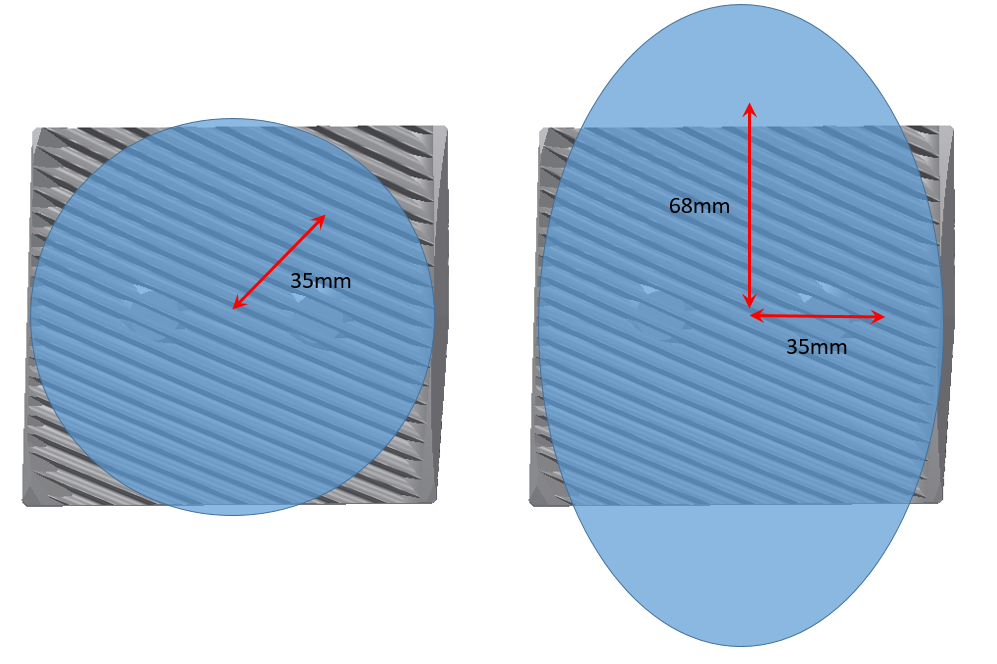
\includegraphics[width=.9\textwidth]{figures/TWOBEAMDISTRI.png}
    \caption{\it Representation of the two ECRH beam heat flux distribution cases}
\end{figure}
\normalsize{\indent The calculation of the integral parameters as well as the analytical calculation of the surface integrals were done on Wolfram Mathematica\textsuperscript{\textregistered} . There are two different cases, one axisymmetric and another non-axisymmetric (elliptical). For the first case, almost all of the power ~99\% hits the ECRH reflector tile. The standard deviation is defined to be 35mm, for debug and validation purposes, 86\% of the power should be included within a disk of radius 35mm. For the elliptical distribution, much less power hits the reflector tile. The distribution properties are also different and feature two different radii, the minor semi-radius and the major semi-radius. Their values are respectively 35mm and 68mm, both of them defining an ellipse. Similarly, to the circular distribution, for debugging, 86\% of the overall power should be included within the area of the ellipse.}
\\
\break
\normalsize{\indent With help of those information, the integration coefficients could be calculated. The first integral was expressed in a cylindrical coordinate system. The first APDL code written by (J. Zhu) in 2019 only featured the circular heat flux distribution and was based on calculations made by Torsten Stange. The integrated function for Gaussian distribution has the form $exp(-2r^2)$. The surface integral can be written:}